%%%%%%%%%%%%%%%%%%%%%%%%%%%%%%%%%%%%%%%%%%%%%%%%%%%%%%%%%%%%%%%%%%%%
%% I, the copyright holder of this work, release this work into the
%% public domain. This applies worldwide. In some countries this may
%% not be legally possible; if so: I grant anyone the right to use
%% this work for any purpose, without any conditions, unless such
%% conditions are required by law.
%%%%%%%%%%%%%%%%%%%%%%%%%%%%%%%%%%%%%%%%%%%%%%%%%%%%%%%%%%%%%%%%%%%%

\documentclass[
  digital,     %% The `digital` option enables the default options for the
               %% digital version of a document. Replace with `printed`
               %% to enable the default options for the printed version
               %% of a document.
%%  color,       %% Uncomment these lines (by removing the %% at the
%%               %% beginning) to use color in the printed version of your
%%               %% document
  oneside,     %% The `oneside` option enables one-sided typesetting,
               %% which is preferred if you are only going to submit a
               %% digital version of your thesis. Replace with `twoside`
               %% for double-sided typesetting if you are planning to
               %% also print your thesis. For double-sided typesetting,
               %% use at least 120 g/m² paper to prevent show-through.
  nosansbold,  %% The `nosansbold` option prevents the use of the
               %% sans-serif type face for bold text. Replace with
               %% `sansbold` to use sans-serif type face for bold text.
  nocolorbold, %% The `nocolorbold` option disables the usage of the
               %% blue color for bold text, instead using black. Replace
               %% with `colorbold` to use blue for bold text.
  lof,         %% The `lof` option prints the List of Figures. Replace
               %% with `nolof` to hide the List of Figures.
  lot,         %% The `lot` option prints the List of Tables. Replace
               %% with `nolot` to hide the List of Tables.
]{fithesis4}
%% The following section sets up the locales used in the thesis.
\usepackage[resetfonts]{cmap} %% We need to load the T2A font encoding
\usepackage[T1,T2A]{fontenc}  %% to use the Cyrillic fonts with Russian texts.
\usepackage[
  main=english, %% By using `czech` or `slovak` as the main locale
                %% instead of `english`, you can typeset the thesis
                %% in either Czech or Slovak, respectively.
  english, german, czech, slovak %% The additional keys allow
]{babel}        %% foreign texts to be typeset as follows:
%%
%%   \begin{otherlanguage}{german}  ... \end{otherlanguage}
%%   \begin{otherlanguage}{czech}   ... \end{otherlanguage}
%%   \begin{otherlanguage}{slovak}  ... \end{otherlanguage}
%%
%%
%% The following section sets up the metadata of the thesis.
\thesissetup{
    date        = \the\year/\the\month/\the\day,
    university  = mu,
    faculty     = fi,
    type        = mgr,
    department  = Department of Machine Learning and Data Processing,
    author      = Bruno Petrus,
    gender      = m,
    advisor     = {Prof. RNDr. John Smith, CSc.},
    title       = {Segmentation of tunneling nanotubes},
    TeXtitle    = {The Proof of $\mathsf{P}=\mathsf{NP}$},
    keywords    = {keyword1, keyword2, ...},
    TeXkeywords = {keyword1, keyword2, \ldots},
    abstract    = {%
      This is the abstract of my thesis, which can

      span multiple paragraphs.
    },
    thanks      = {%
      These are the acknowledgements for my thesis, which can

      span multiple paragraphs.
    },
    bib         = biblio.bib,
    %% Remove the following line to use the JVS 2018 faculty logo.
    facultyLogo = fithesis-fi,
}
\usepackage{makeidx}      %% The `makeidx` package contains
\makeindex                %% helper commands for index typesetting.
%% These additional packages are used within the document:
\usepackage{paralist} %% Compact list environments
\usepackage{amsmath}  %% Mathematics
\usepackage{amsthm}
\usepackage{amsfonts}
\usepackage{url}      %% Hyperlinks
\usepackage{markdown} %% Lightweight markup
\usepackage{listings} %% Source code highlighting
\usepackage{subcaption}
\lstset{
  basicstyle      = \ttfamily,
  identifierstyle = \color{black},
  keywordstyle    = \color{blue},
  keywordstyle    = {[2]\color{cyan}},
  keywordstyle    = {[3]\color{olive}},
  stringstyle     = \color{teal},
  commentstyle    = \itshape\color{magenta},
  breaklines      = true,
}
\usepackage{floatrow} %% Putting captions above tables
\floatsetup[table]{capposition=top}
\usepackage[babel]{csquotes} %% Context-sensitive quotation marks
\begin{document}
%% The \chapter* command can be used to produce unnumbered chapters:
\chapter*{Introduction}
%% Unlike \chapter, \chapter* does not update the headings and does not
%% enter the chapter to the table of contents. I we want correct
%% headings and a table of contents entry, we must add them manually:
\markright{\textsc{Introduction}}
\addcontentsline{toc}{chapter}{Introduction}

Theses are rumoured to be \enquote{the capstones of education}, so
I decided to write one of my own. If all goes well, I will soon
have a diploma under my belt. Wish me luck!
[TODO: explain semantic segmentation] 

\chapter{Data}
The data which we use was taken by our Estonian partners, the data comes from a
sample of wings of the *Drosophila* fly. 

Our work begun when the Estonian partners send us the four different datasets of
the wanted to study phenomena. To study the effects of tunneling nanotubes which
are these thin, long and often time curved structures, they deciced to use wings
of fly larvae. A schematic can be viewed in Figure [TODO]. This is quite
interesting sample as it generaly has, as can be seen in Figure [TODO] and
[TODO] two distinct layers of cells, between which a vertical pillar like
structures are visible. These structures are what we will refer to in this work
as pillars for simplicity. These belong to the [FINISH] part of the wings. How
such data can be acquired and for more information of the process I recommend
looking into the \parencite{Tran2024Programmed} paper.

\section{Acquired Datasets}

The data was captured using fluorescence microscopy. [TODO simple explanation]
and four distinct datasets were acquired. Three of these datasets were captured
with two different channels, larger volume and smaller spatial resolution. All
the datasets are actually part of a time series as it is of quite interest in
looking at the temporal properties of the biological phenomena i.e. do tunnels
stay for multiple steps or are they short-lived? Does their properties change in
time? But that was not the main point of our current research.

The last dataset contains just one channel. The fluorescent dye was selected to
highligh both the pillars and the tunnels as can be seen in Figure [TODO]. As we
can see unlike the previous datasets this was capture at much higher spatial
resolution; therefore, we can see that the dye react mostly in the cell membrane
and they appear hollow. Moreover, the tunnels are much more visible compared to
the previous three datasets, but it only contains a single channel now.

As said before the data was captured by our Estonian partners at [TODO], to
further propel the research they promised us to annotate the three large
datasets, but after several months no labels were given which complicated the
research and work. Hence, we approached our collegues at [TODO what fac.] and
they were kind enough to help us. As we only have labeles to one dataset, in the
rest of this work we will be primarily 

\begin{figure}
    \begin{center}
        \includegraphics[width=0.6\linewidth]{resources/t017z0_saturated1percent.png}
    \end{center}
    \caption{First slice of the data at time step 17, after the biologist
    preprocessing pipeline}.
    \label{fig:biologistpreprocessing}
\end{figure}

\section{Labelling and preprocessing}

The biologist created a protocol which they followed by annotating the samples.
They decided to preprocess the data by converting the images from 16bit
grayscale image into 8bit grayscale images, then a 1\%-percentile stretch was
applied to further enhance the images. The result of the preprocessing is
visible in Figure \ref{fig:biologistpreprocessing}. As can be seen on the figure,
this makes the tunnels easier to see at the cost making noise more visible.

\begin{figure}
    \centering
    \begin{subfigure}[b]{0.45\textwidth}
        \centering
        \includegraphics[width=\linewidth]{resources/mask000-slice3-saturated.png}
        \caption{}
        \label{fig:gt-slice-3}
    \end{subfigure}\hfill
    \begin{subfigure}[b]{0.45\textwidth}
        \centering
        \includegraphics[width=\linewidth]{resources/mask000-slice3-composite.png}
        \caption{}
        \label{fig:gt-slice-3-composition}
    \end{subfigure}
    \caption{Labeled tunnels by a biologist at 0th time slot on the left. On the
    right the binarized version can be seen overlaid on top of the original
    data.}
    \label{fig:gt-slice-3}
\end{figure}

After the preprocessing is done, the protocol states that picking random time
slots at least 100 instances of tunnels must be annotated, and each frame has to
be fully annotated. According to this protocol the biologists picked two time
steps --- the 0th and 17th step ---  and gave us uniquelly labeled data. The
ground truth created by a biologist for the 0th time slot is visible in the left
part of Figure \ref{fig:gt-slice-3}. In the right part of the mentioned figure
a composition was created with gray data and the binarised ground truth in
magenta colour.

\begin{figure}
    \begin{center}
        \includegraphics[width=0.6\linewidth]{resources/duplicatedlabel.png}
    \end{center}
    \caption{Maximum projection of the data highlighting problematic tunnel with id 32 located in bottom right quadrant}.
    \label{fig:duplicatedlabel}
\end{figure}

Afterwards the labels were check manually and two cases of label duplicity were
found and fixed, by assigning a unique number to the new connected component.
The flawed labels were 33 located in top right quadrant and label 32 located
bottom right quadrant as can be seen in Figure \ref{fig:duplicatedlabel}.

\chapter{Architectures}
This chapter deals with what neural network architectures were used in
developing the solution.

\section{Preliminary research}
We began by researching similar papers dealing with segmenting nanotubular
structures. Two promising papers we found are ..[TODO]. In

\parencite{Hodneland2006Automated} the researchers are similar to use dealing
with tunnels between cells, but in their case the tunnels form a long straight
lines. In the paper they describe a multistep algorithm which takes employ two
channels, one is for segmenting cell borders and tunnels, while in the other
channel the cells inside are much more visible, hence, this can be used to
better separate cells and tunnel.

As our data has different modality, this approach could not be used. They also
assume that the tunnels are straight which is not true in our case.
The other paper which specificaly mentiones tunneling nanotubes is
\parencite{Ceran2022TNTdetect}. This paper provides consists of three parts.
They describe how to improve the labels and make it easier 

\section{U-Net}
\label{sec:unet}

In 2015 a seminal paper by Rossenberger et al. \parencite{Ronneberger2015} was
published dealing with semantic segmentation of medicine data. The paper
achieved impressive results with very limited dataset. The neural network
architecture is called U-Net and has been behind many models later to come.
[TODO citation]

\begin{figure}
    \begin{center}
        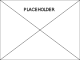
\includegraphics[width=0.6\linewidth]{resources/placeholder.png}
    \end{center}
    \caption{A UNet architecure diagram}.
    \label{fig:unetdiagram}
\end{figure}

The key architectural part of the U-Net lays in the introduction of transposed
convolution layers which upsample the result of the encoder. This is placed
after what traditionally like in the neck in VGGNet [TODO citation] was followed
by a classification head now follows the decoder. A diagram can be seen in
Figure \ref{fig:unetdiagram}. As can be seen in the figure, on input it takes an
image and it is followed by a horizontal block formed of two convolutions,
followed by a max pool operation which downsamples the image by a factor of 2.
After this is done numerous times, which depends on the depth of the network set
by the user, additional convolution is applied. The results of the neural
network before the downsample operation is taken is also saved. After the neck
part a series of upsampling operations take place. This is achieved using a
transposed convolution operation and the weights are learned automatically by
the network. Note that other possibilities, like using interpolation in [TODO
citation] was not researched in this work. This upsampling operation doubles the
spatial resolution at the cost of halving the number of channels. Each time such
operation takes place the result of relevant encoder layer is concatonated,
followed by two additional convolutions. Finally we do a final convolution
operation to ouput the right amiunt of classes, which in our case is equal to
two (tunnel or BG/pillar).

The two main reasons for choosing this architecture compared to other was that
the U-Net architecure is well estabilished, widely used, achieves good
performance [TODO citation], but mainly due its nice property that Rossenberger
et al. \parencite{Ronneberger2015} demonstrated that you do not need a huge
dataset to teach the neural network. As our data is quite limited in terms of
size this is a very usefull feature.

The Figure \ref{fig:unetdiagram} is visualising how the UNet architecure can be
used to train a 2D model, but there is not reason why we could not use 3D
versions of convolution, maxpool and transposed upconvolution. 

\subsection{Anisotropic U-Net}

In machine learning it is often tried to increase the model depth to improve the
perfomance of the neural network. This is of course not true universaly as this
can make the network harder to train can cause the network to overtrain [TODO
citation needed]. Since our data is heavily anisotropic we are limited in how
much we can downsample in the z direction, as we have only 7 voxel inside the z
dimension, it is possible to downsample just two times before reaching depth
equal to 2. Moreover, it would probably be reasonable to assert that compressing
all the depth information into a single channel is asking the neural network to
do a lot of work compressing the info.

This problem motivated us to create a new version of the U-Net which uses
anisotropic kernels instead of isotropic kernels for both convolution and the
maxpool operation.

\begin{figure}
    \begin{center}
        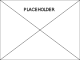
\includegraphics[width=0.6\linewidth]{resources/placeholder.png}
    \end{center}
    \caption{Visualisation of 3D convolution and maxpool operation}.
    \label{fig:visanisooperations}
\end{figure}

As is ilustrated in Figure \ref{fig:visanisooperations} a 3D convolution
uses a 3D kernel to look into a 3D part of the input. By appriopriately padding
the output, we can keep the same dimension in the z axis. Moreover, to prevent
early downsampling in the z dimension we can use anisotropic versions of these
operators. Instead of downsampling by a factor of 2 in all directions, we can
ignore downsampling in the z dimension by setting the kernel size in that
direction equal to 1 [TODO or 0?].

\section{The CSAM module}

This section talks about the channel and spatial attention module (further
refered to as the CSAM) mentioned in the CS-Net paper \parencite{Mou2021}. In
this paper the author tried to improve the performance of UNet architecture by
incorporating attention into the model. This was motivated by using the
architecture for segmenting blood vessels and related biological features and
seeing that one of the problems which was often encoutnered is the fact that
these network had trouble connecting faint blood vessels leading to a
connectivity issues. The attention models helps with connecting them together.

Even though we are not dealing with vessels in our case, the tunnels do visually
resemble some curvilinear structures. We also encountered some of these issues
with connectivity, and as such this might also alleviate the our problems [TODO
reference].

\begin{figure}
    \begin{center}
        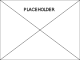
\includegraphics[width=0.6\linewidth]{resources/placeholder.png}
    \end{center}
    \caption{The CSAM module from Paper [TODO CITE]}.
    \label{fig:csammodule}
\end{figure}

The Figure \ref{fig:csammodule} by \parencite{Mou2021} explain the working
principle behind the CSAM module. It is formed of two paths, the spatial
attention block SB and the channel attention block CAB. One is designed to help
the network find tubular structures inside the spatial direction while the other
is used for helping the network learn inter-channel dependency.

\subsection*{SAB}
The design is motivated by the detection of tubular structures such as blood
vessels in retina images. The detection of such features might require
contextual information rather than purely local information. This lead the
author to use anisotropic kernels 

\subsection*{CAB}
The design ...



\section{Squeeze and excitation block}
In Paper \parencite{Hu2018} researchers demonstrated how a simple small block
can be inserted inside deep neural networks to improve their performance accross
various datasets and tasks. The researchers postulate that this block helps the
network learn inter channel dependecies [TODO where in paper].

\begin{figure}
    \begin{center}
        \includegraphics[width=0.6\linewidth]{resources/t017z0_saturated1percent.png}
    \end{center}
    \caption{Squeeze and exciation block from Paper \parencite{Hu2018}}
    \label{fig:se_diagram}
\end{figure}

The general principle of a squeeze and excitation block is illustrated in Figure
\ref{fig:se_diagram}. The main idea is that we let the network learn
significance of each channel. This is technically done by multiplying the data
$U$ by a number from 0 to 1 in each channel separately.

The squeeze and excitation block consists of four operations: truncate, squeeze,
excitation, and scaling. The truncate operation shown as $F_{TR}$ is a general
convolution operator, which reduces the dimension. This step is not crucial in
the scheme, but it is mainly to illustrate the point, that SE block is usually
built upon some operation. More importantnly, the transdormed data is taken and
run through a squeeze operation, which basically does some global operation in the
whole channel. After that, the excitation operation comes. This operation was
designed to have the following properties: they wanted to create a flexible
operation --- meaning an operation capable of learning non-linear dependecies
--- and they wanted it to be non-mutually exclusive between channels. This is
done by applying two convolutions followed by ReLU and sigmoid respectively.
Note that the first convolution produces output with less than the original
number of channels and the ratio is called the reduction factor. Finally the
last convolution expands the number of channels to the original size. The
comvination of squeeze and excitation allows the network to learn how to weight
each channel (the scale operation mentioned above) by considering multiple
channels.

\begin{figure}
    \begin{center}
        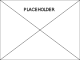
\includegraphics[width=0.6\linewidth]{resources/placeholder.png}
    \end{center}
    \caption{Placement of SE blocks inside the U-Net by \parencite{Rundo2019}}
    \label{fig:se_unet}
\end{figure}

Another issue is where to put this block, as I already mentioned the truncate
operation, the authors suggest placing it after applying convolution, they also
suggest placement in the Inception and ResNet blocks [TODO citation?]; however,
placement inside a UNet architecture is not mentioned. After further
considerations [TOOD what options] the blocks were placed according to Paper
\parencite{Rundo2019} after every step in the decoder and after each upsampling
step as is shown in Figure \ref{fig:se_unet}.

\chapter{Training}
This chapter explains how the aforementioned neural networks were trained. How
the data was split and handled.

\section{Processing data}
\label{sec:processing_data}
[TODO mention alternatives to supervised learning somewhere]

As mentioned in the previous Chapter [TODO cite], we have 2 time frames of
7x512x512 voxels. As we in some sense only have 2 full images the splitting of
the dataset proved somewhat complicated. We wanted to experiment with using full
3D U-Nets therefore using full sized images would lead to using just one image
for training and one for testing. However, it is no reasoanble to think that
this would be enough to teach the network any reasonable decision. As already
mentioned in Chapter \ref{sec:unet} a nice feature the U-Net architecture is
that it can be learned on much smaller datasets as was demonstrated in the
original U-Net Paper \parencite{Ronneberger2015} [TODO check] and also in the
CS-Net paper \parencite{Mou2021} were few dozens of images were used to train a
neural network to segment medical images. As such a way to extract about a
hundred images was needed.

Splitting the dataset into quadrants would still yield only about 8 7x256x256
images. Importantly, we have about 150 [TODO check] labeled tunnels, which would
suffice the needed number of images. Hence, we decided to cut out the tunnels
and train the network on the these subparts. Note that we still need to run the
network on the whole images, but for training purposes this will suffice.

The splitting logic iterates through every single tunnel and cuts it out. As the
tunnels have different sizes we decided to cut out the bounding boxes of the
tunnels with a set of minimum size. For the minimum size we decided to go for a
7x90x90 shape as that confortably fits majority of tunnels and provides a decent
context around it. [TODO mention expansion after explaining the splits]

\begin{figure}
    % TODO: replace with nicer image.
    \begin{center}
        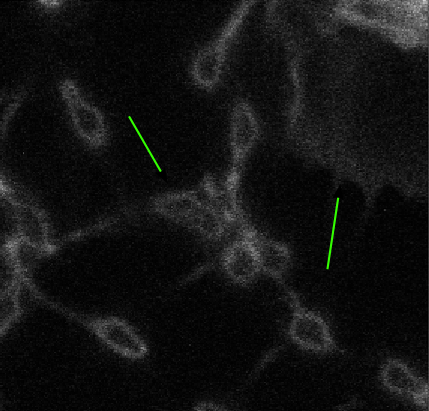
\includegraphics[width=0.6\linewidth]{resources/tmp/t017_upperright.png}
    \end{center}
    \caption{}
    \label{fig:upperright}
\end{figure}

It is still important to be somehow able to split the dataset into the train,
test and evalution subset. As the dataset is quite limited choosing a random
sybpart to evaluate the perfomance is not ideal. The various parts of the
dataset do not have the same number of tunnels, tunnels of the same morphology
and the same amount of noise and irrelevant structures. For example in the upper
right corner in Figure \ref{fig:upperright} we can find some irrelevant
structures which are not present in the rest of the dataset.

%As somehowe quantifying the ideal split would be a very demanding task we 
Somehow quantifying the ideal split would be a very challenging and unclear task
so we are always doing something similar to a leave one out [TODO cite] cross
validation. Each time four different models are trained and in each run a
different quadrant is considered to be the testing subset and the remaining
three quandarnt are used for training the model.

This is still quite challenging to do properly as not every tunnel lies neatly
inside one of the quadrants. A split that is used in training is visualised in
Figure [TODO] where a possible split is shown in two colours.

The decision if a particular tunnel belongs in test or train subset is made by
the following decision. [TODO check the numbers and finalise this section.]

\section{Training}


\subsection{Loss funtions}
Since we can look at finding tunneling nanotubes as a binary classification
problem applied at every pixel, it naturally comes to use a binary cross-entropy
loss to teach the network to learn to segment the images. However, our dataset
is very heavily imbalanced as the data contains a lot more negative examples. To
somewhat help the training to pay more attention to the tunnels, the
cross-entropy was weighted by a factor or 50, which was estimated by taking the
calculating the ration of pixels classified as background and pixels assigned to
some tunnel by the biologist.

To further improve the performance of the training, we got inspired CS-Net paper
which uses Dice loss, and some papers claim that the combination of Dice loss
and cross-entropy loss lead to better performance in many segmentation tasks
\parencite{ma2020segmentationlossodyssey}. By using Dice loss it is meant to
optimize the value of the Dice coefficient. This is defined as taking
$L_{Dice} = 1 - \text{Dice}$, meaning that as we get segmentation results closer
to the ideal mask, we get closer to 0.

% TODO: full loses



For the loss function we were inspired by [TODO cite
the loss paper] and by CS-Net \parencite{Mou2021} to try a mix of Dice loss anda
binary cross-entropy loss. Since we were not sure about how to weight these
losses we went by setting their weights to be equal. 

To somewhat alleviate the
issue with the uneven positive and negative labels in the labels, we counted how
many positive and how negative pixels are in the whole dataset, and arrived at
a 50 [TODO check] ratio of these two classes.

[TODO defi. of CE]
[TODO defi. of Dice]
[TODO defi. of Jaccard]

\subsection*{Optimizers, learning rates, regularization}
The neural network was trained using Adam optimzizer, but soon switched as we
are also using weight decay, equal to 1e-4, it is commonly advised to use the
AdamW variant as it correctly decouples the weight decay from the gradient
updates \parencite{loshchilov2019}. However, in practice no vast effect was
observed during out testing.

During the development of the training loop we observed that setting the
learning rate to 0.001 [TODO check] and weight decay to [TODO check] achieved a
very stable learning. This was when using smaller windows size, and the overall
loop was not quite as robust; however, as the development progress the learning
stayed well behaved and no experimentation on the values was done. Since the
Adam family of optimizers change the learning rate adaptively per neuron we did
not see the benefit of rerunning all evaluations also for different learning
strategies considering the time requirements to perform such a study.

\subsection*{Training the network}

As was mentioned in Section \ref{sec:processing_data} the overall size of the
dataset was rather tiny compromising of just a few images. To alleviate this we
instead started focusing on training a network on smaller patches of 7x64x64
size.

A common problem with training neural networks is their capacity to overtrain
on the training part of the dataset. This often times leads to poor
generalisation performance. This is especiialy true fro really small datasets
such as ours. One of the common ways to deal with this problem, as is mentioned
in the original U-Net paper is the use of augmentations
\parencite{Ronneberger2015} to artificially enlarge the training set. In our
case we decided that we will use only augmentations which do not require
interpolation. The reason is that unlike many other tasks, we are potentially
dealing with quite thin structres, which could easily be significantly supressed
or blured and no longer be seen.

In each batch, a different set of transforms are used. This works by setting a
random probability of this particular transform to be applyied. For the training
we are:
\begin{itemize}
    \item{Adding random noise with a Gaussian distribution of mean 0 and 0.01
        standard deviation with probability 0.5, which adds very faint noise.
        This is a relatively low amount of noise and was chosen during the
        development of the network as we did not want to change the images to
        look completely different to the orignal ones.}
    \item{Random flipping in every axes.}
    \item{Random spatial crop which always crops to the preset size 7x64x64 from
        any other size.}
\end{itemize}
A possible problem of using small tiles centered at tunnels is that we might
introduce unwanted bias into the network, as it might learn to always try to
find the tunnel in the middle. The design designation behind using random
spatial crop was to try to suppress this, as the program now randomly finds a
crop of the wanted size, which reduces this problem.

Given all the mentioned settings the 


% [TODO mention inside the intro chapter or architecture]
% When training
%networks using supervised learning approach we usualy have hundreds or more
%images [TODO CITE SOME classification papers], which we unfortunately do not
%have. But, one of the nice 

%it is not possible to simply use one timeframe for training
%and one for testing 

%splitting and stuff
how the neural networks were trained.

\chapter{Implementation}


\section{Used technologies}
Python, mlflow, Bash, uv, the shuffling, setting explicit seeds, issues with
batch vs loss, implementing the loss functions in pytorch
implementing the squeeze and excitation.

\section{Environment}

\subsection{Justification for the used technologies}
The previously described training and preprocessing in previous chapters was
implemented as collection of Bash scripts, python scripts and a python module.
All of the code is available as part of the master thesis alongside several of
the trained networks for the user.

The Python environment is packaged and its dependecies are resolved by a tool
cold uv \parencite{uv} developed by a company called Astral, who specialises on
creating modern automatic tooling for Python. The environment is described using
a TOML file available and list a number of dependencies. Altough the project is
quite recent compared to others like Poetry, uv is significanlty faster.

For convenience I am also including a \texttt{requirements.txt} which was automatically generated
from a virtual Python environemnt, but the officially supported version is using
the uv package manager. The environment can then be created in two ways: if the
user runs a computer with a GPU, the working environmnet is creating using the
command \texttt{uv sync --extra torch-gpu} which assumes that CUDA version 12.4
is installed.

I decided to use Python to develop the training and evaluation scripts, while
handling the pipelines around it with Bash. Altough Python is an interpreted and
dynamically typed language and therefore is comparably slower than other lower
level languages traditionally used in image processing like C++, its nature
allows it to rapidly prototype new application. Moreover, many packages call
code written in other languages such as C++, Fortran or C, to somewhat alleviate
the performance problem. Lastly, Python has become a widely adopted language in
the area of neural networks, and many researchers publish their code in Python.

As was already mentioned even though the majority of code is written in Python
it is quite cumbersome to create a single Python script which handles both
training and evaluation, especially if something changes in one of them. This
fundamentally breaks the famous principle in software architecture called the
separation of concers. As such a bash script is provided in the code archive
under \texttt{scripts} called \texttt{run.sh} which is the main entrypoint for
running the code.

As a lot of the evaluation is concerned with doing proper cross-validation and
then averaging the results it was easier to create a script which is easily
configured using a text editor or by providing and parsing CLI arguments and the
averaging and choosing different datasets should not be a responsibility of the
Python script. As such, creating directories, running code, aggregating results
and parsing arguments is a natural job for a scripting language such as Bash.
The obvious disadvantage is that it is limited to the Unix and Unix like
operating systems.

As for the other tooling, here I list the most important tools:
\begin{itemize}
    \item{MLflow is tool for handling machine learning pipelines, it allows to
        track experiments, compare results, save and load models, deploy models
        etc. In this work it was used to create a nice interface to keep track
        of various experiments.}  % cite https://mlflow.org/docs/latest/ml/
    \item{ruff linter TODO cite is an extremely fast Python linter which was
        developed by the company Astra. It automatically formats code and can
        even fix some of the basic lint errors.}
    \item{numpy TODO CITE has become one of the fundamental packages in
        scientific computing in Python ecosystem. It provides a very efficient
        implementation of} 
    \item{scikit-learn provides a great framework for building machine learning
        models not just deep learning models. This was used mainly for splitting
        datasets and using their framework for handling batching.}  % TODO: https://scikit-learn.org/stable/index.html
    \item{scikit-image is a package providing various algorithms for processing
        images e.g. segmentation algorithms, point transform, mathematical
        mopohlogy. I used it to handle the post-processing of masks and to find
        connected components.} % TODO: https://scikit-image.org/
    \item{Pytorch is a popular deep learning framework with focus on flexibility
        and speed, this allows the user to create a well performing neural
        network very fast. It automatically creates computational graphs
        allowing it to compute gradient upgrades efficiently. It handles
        connecting to various hardware like CPU and GPUs automatically. This has
        allowed PyTorch to become one of the most used packages in the Python
        ecostsem and is why I chose it to develop the program. TODO CITE} % https://pytorch.org/projects/pytorch/ 
    \item{MONAI is another opensource framework for building neural networks on
        top of PyTorch. It focuses on building models used in Medical area. In
        the project I was using this package to handle augmentations of the
        dataset as it provides first class support for 3D data.} % cite https://github.com/Project-MONAI/MONAI
    \item{matplotlib}
\end{itemize}

\section{Use case modelling and expected usage}
Here describe how to call the run.sh
We identified two particular use cases for the application, it should provide a
reasonably easy interface for training and then an interface for evaluating the
models given some training data. For this purpose a single Bash script called
wasc created which serves the 

\section{Loss and metrics implementation}

\section{SE implementation}

\section{NN implementation}

\section{Postprocessing}

\chapter{Evaluation}
how we evaluate the networks

\section{Choice of depth}

\section{Choice of overlap}

\section{Different architectures}

\section{Recommended values}

\section{Ablation studies}

\chapter{Discussion}
what to do next

\end{document}
